% =====================================================================
% BMED365: Patient Similarity Networks (PSN)
% Beamer-presentasjon - Topic List P01-P08
% =====================================================================
\documentclass[aspectratio=169, 10pt]{beamer}

% =====================================================================
% PACKAGES
% =====================================================================
\usepackage[utf8]{inputenc}
\usepackage[T1]{fontenc}
\usepackage[english]{babel}
\usepackage{graphicx}
\usepackage{tikz}
\usetikzlibrary{shapes.geometric, arrows, positioning, calc}
\usepackage{booktabs}
\usepackage{amsmath}
\usepackage{fontawesome5}
\usepackage{hyperref}
\hypersetup{colorlinks=true, linkcolor=blue, urlcolor=blue}
\usepackage{amssymb}

% =====================================================================
% THEME AND COLORS
% =====================================================================
\usetheme{Madrid}
\usecolortheme{beaver}

% Colotherwise for TikZ diagrams
\definecolor{uibblue}{RGB}{0, 61, 115}
\definecolor{uibred}{RGB}{175, 28, 44}

% =====================================================================
% TITLE INFO
% =====================================================================
\title{Patient Similarity Networks (PSN)}
\subtitle{BMED365: Topic List P01--P08}
\author{BMED365}
\date{Spring 2026}

% =====================================================================
% DOCUMENT
% =====================================================================
\begin{document}

% Title page
\begin{frame}
    \titlepage
\end{frame}

% Table of Contents
\begin{frame}{Overview}
    \begin{enumerate}
        \item \textbf{Fundamentals of PSN}
        \begin{itemize}
            \item P01: Explain the concept of patient similarity networks (PSN)
            \item P02: Describe how PSN can support precision medicine
        \end{itemize}
        \item \textbf{Similarity Calculation}
        \begin{itemize}
            \item P03: Calculate similarity between patients
            \item P04: Construct a PSN from a patient-feature matrix
            \item P05: Choose threshold value for edge creation in PSN
        \end{itemize}
        \item \textbf{Analysis of PSN}
        \begin{itemize}
            \item P06: Identify patient subgroups via community detection
        \end{itemize}
        \item \textbf{Advanced Topics}
        \begin{itemize}
            \item P07: Advantages and limitations of the PSN approach
            \item P08: Multimodal PSN (integration of different data types)
        \end{itemize}
    \end{enumerate}
\end{frame}

% =====================================================================
% SECTION: Fundamentals of PSN
% =====================================================================
\section{Fundamentals of PSN}

\begin{frame}{P01: Explain the concept of \href{https://en.wikipedia.org/wiki/Patient_similarity_network}{patient similarity networks (PSN)}}
    \begin{columns}[T]
        \begin{column}{0.55\textwidth}
            \textbf{What is a patient similarity networks?}
            \begin{itemize}
                \item En \textbf{graf} der hver node representerer en patient
                \item \textbf{Kanter} forbinder patienter som ligner hverandre
                \item Likhet basert på clinicale variabler (symptoms, vitalia, demografi), biomarkerer, genethics, avbildning, livsstilsfakcountser
            \end{itemize}
            
            \vspace{0.2cm}
            \textbf{Main idea:}
            \begin{itemize}
                \item Pasienter med lignende profiler grupperes sammen
                \item Avdekker naturlige subgrupper i patientpopulasjonen
                \item Grunnlayers for \textbf{patient-stratifisering}: identify undergrupper med felles egenskaper for goalrettet treatment
            \end{itemize}
            
            \vspace{0.2cm}
            \scriptsize\textbf{Sentrale referanser:}
            \href{https://doi.org/10.1038/ncomms5022}{Pai \& Bader (2018)},
            \href{https://doi.org/10.1093/jamia/ocw154}{Li et al. (2015)}
        \end{column}
        \begin{column}{0.42\textwidth}
            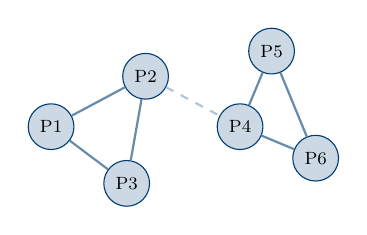
\begin{tikzpicture}[scale=0.8, transform shape]
                \tikzstyle{patient} = [circle, draw=uibblue, fill=uibblue!20, minimum size=0.7cm, font=\footnotesize]
                \tikzstyle{edge} = [draw, thick, uibblue!60]
                
                \node[patient] (p1) at (0,0) {P1};
                \node[patient] (p2) at (1.5,0.8) {P2};
                \node[patient] (p3) at (1.2,-0.9) {P3};
                \node[patient] (p4) at (3,0) {P4};
                \node[patient] (p5) at (3.5,1.2) {P5};
                \node[patient] (p6) at (4.2,-0.5) {P6};
                
                \draw[edge] (p1) -- (p2);
                \draw[edge] (p1) -- (p3);
                \draw[edge] (p2) -- (p3);
                \draw[edge] (p4) -- (p5);
                \draw[edge] (p4) -- (p6);
                \draw[edge] (p5) -- (p6);
                \draw[edge, dashed, uibblue!30] (p2) -- (p4);
            \end{tikzpicture}
            
            \vspace{0.3cm}
            \footnotesize\textit{To patientgrupper med sterk intern likhet}
        \end{column}
    \end{columns}
\end{frame}

\begin{frame}{P02: Describe how PSN kan støtte \href{https://en.wikipedia.org/wiki/Precision_medicine}{precision medicine}}
    \begin{block}{Precisionsmedisin}
        Tilpasse treatment til den individuelle patienten basert på deres unike profil -- ikke ``one size fits all''
    \end{block}
    
    \vspace{0.3cm}
    \textbf{PSN støtter precision medicine ved å:}
    \begin{enumerate}
        \item \textbf{Identifisere subgrupper} -- Finne patienter med lignende diseasesmekanismer
        \item \textbf{Predikere treatmentsrespons} -- ``Pasienter som ligner deg responderte godt på X''
        \item \textbf{Oppdage ukjente sammenhenger} -- Avdekke mønstre på tvers av datatyper og etablerte diagnosisr
        \item \textbf{Integrere heterogene data} -- Kombinere klinikk, omikk, avbildning
    \end{enumerate}
    
    \vspace{0.3cm}
    \begin{alertblock}{Example: IBS-studien}
        I Lab 1 bruker vi PSN på IBS-patienter to undersøke sammenhenger mellom mage-tarmsymptoms, hjerneavbildning (MRI) og kognitive funksjoner.
    \end{alertblock}
\end{frame}

% =====================================================================
% SECTION: Similarity Calculation
% =====================================================================
\section{Similarity Calculation}

\begin{frame}{P03: Calculate likhet (\href{https://en.wikipedia.org/wiki/Similarity_measure}{similaritet}) mellom patienter}
    \textbf{Vanlige similaritets-/avstandsgoal:}
    \vspace{-1mm}
    \begin{columns}[T]
        \begin{column}{0.48\textwidth}
            \textbf{Euklidsk avstand ($\ell_2$):}
            \vspace{-2mm}
            \[
            d_E = \sqrt{\sum_{i=1}^{n}(x_i - y_i)^2}
            \]
            \vspace{-3mm}
            \footnotesize
            \begin{itemize}\setlength{\itemsep}{0pt}
                \item Rett linje mellom punkter i $\mathbb{R}^n$
                \item Følsom for scale
                \item God for kontinuerlige data
            \end{itemize}
            \normalsize
            
            \textbf{Manhattan avstand ($\ell_1$):}
            \vspace{-2mm}
            \[
            d_M = \sum_{i=1}^{n}|x_i - y_i|
            \]
            \vspace{-3mm}
            \footnotesize
            \begin{itemize}\setlength{\itemsep}{0pt}
                \item ``Bykvartal''-avstand
                \item Mer robust mot uteliggere
            \end{itemize}
        \end{column}
        \begin{column}{0.48\textwidth}
            \textbf{Gower-avstand:}
            \vspace{-2mm}
            \[
            d_G = \frac{1}{n}\sum_{i=1}^{n}d_i(x_i, y_i)
            \]
            \vspace{-1mm}
            \scriptsize
            \textit{$d_i$ = normalisert avstand for variabel $i$:}
            
            \vspace{0.5mm}
            num.: range-norm., kat.: 0/1, binær: id.
            
            \vspace{1mm}
            \footnotesize
            \begin{itemize}\setlength{\itemsep}{0pt}
                \item Håndterer \textbf{blandede datatyper}
                \item Normaliserer automatic
                \item Ideell for clinicale data!
            \end{itemize}
            
            \begin{block}{\scriptsize Konvertering}
                \scriptsize $\text{similaritet} = 1 - \text{avstand}$ (norm. til [0,1])
            \end{block}
        \end{column}
    \end{columns}
\end{frame}

\begin{frame}{P04: Construct a PSN from a patient-feature matrix}
    \textbf{Steg-for-steg prosess:}
    
    \begin{enumerate}
        \item \textbf{Organiser data:} Pasient $\times$ Feature-matrise
        \begin{center}
            \scriptsize
            \begin{tabular}{l|cccccc}
                \toprule
                Pasient & Alder & Kjønn & BMI & Blodtrykk & Symptom-score & Biomarkør \\
                \midrule
                P1 & 45 & K & 24.5 & 120/80 & 7 & 1.2 \\
                P2 & 42 & K & 25.1 & 118/78 & 8 & 1.1 \\
                P3 & 67 & M & 31.2 & 145/95 & 3 & 2.8 \\
                \bottomrule
            \end{tabular}
        \end{center}
        
        \item \textbf{Normaliser/standardiser:} Gjør variabler sammenlignbare\\
        \scriptsize (z-score: $(x-\mu)/\sigma$, min-max: $(x-\min)/(\max-\min)$)
        \normalsize
        
        \item \textbf{Beregn similaritetsmatrise:} Alle par av patienter
        
        \item \textbf{Velg threshold value:} Bestem når to patienter er ``like nok''
        
        \item \textbf{Opprett kanter:} Forbind patienter med similaritet $>$ terskel
        
        \item \textbf{Bygg graf:} Bruk NetworkX to layerse nettverket
    \end{enumerate}
    
    \begin{block}{\footnotesize Python-kode (conceptual)}
        \footnotesize
        \texttt{G = nx.Graph()} \\
        \texttt{for i, j: if similarity[i,j] > threshold: G.add\_edge(i,j)}
    \end{block}
\end{frame}

\begin{frame}{P05: Velge \href{https://en.wikipedia.org/wiki/Threshold_model}{threshold value} for edge creation i PSN}
    \begin{block}{\footnotesize Definition}
        \footnotesize \textbf{Terskel} $\tau$: Kant opprettes mellom patient $i$ og $j$ hvis similaritet $s_{ij} > \tau$.
    \end{block}
    
    \vspace{1mm}
    \textbf{Challengeen} (threshold selection er \textbf{critical} for utfall og interpretation):
    \begin{itemize}\setlength{\itemsep}{0pt}
        \item For lav terskel $\rightarrow$ For mange kanter, alle patienter koblet
        \item For høy terskel $\rightarrow$ For få kanter, isolerte noder
    \end{itemize}
    
    \vspace{1mm}
    \textbf{Strategier for threshold selection:}
    \begin{enumerate}\setlength{\itemsep}{0pt}
        \item \textbf{Persentilbasert:} Behold topp 5--10\% av kantene
        \item \textbf{k-nærmeste naboer (k-NN):} Hver node kobles til k nærmeste
        \item \textbf{Statistisk terskel:} $\mu + 1.5\sigma$ av similaritetsadvantageingen
        \item \textbf{Visuell inspeksjon:} Prøv ulike valueer og visualiser
    \end{enumerate}
    
    \vspace{1mm}
    \begin{columns}[T]
        \begin{column}{0.48\textwidth}
            \begin{alertblock}{\scriptsize For mange kanter}
                \scriptsize Mister subgruppestruktur, vanskelig å interpret
            \end{alertblock}
        \end{column}
        \begin{column}{0.48\textwidth}
            \begin{alertblock}{\scriptsize For få kanter}
                \scriptsize Mister informasjon, fragmentert nettverk
            \end{alertblock}
        \end{column}
    \end{columns}
\end{frame}

% =====================================================================
% SECTION: Analysis of PSN
% =====================================================================
\section{Analysis of PSN}

\begin{frame}{P06: Identifisere patient subgroups via \href{https://en.wikipedia.org/wiki/Community_structure}{community detection}}
    \begin{columns}[T]
        \begin{column}{0.58\textwidth}
            \textbf{Community detection i PSN:}
            \begin{itemize}\setlength{\itemsep}{0pt}
                \item Finner naturlige grupperinger av patienter
                \item Pasienter i samme gruppe ligner hverandre mer enn de ligner andre
            \end{itemize}
            
            \vspace{2mm}
            \textbf{Louvain-algoritmen (fra N09):}
            \begin{enumerate}\setlength{\itemsep}{0pt}
                \item Optimaliserer \textbf{modularitet} -- intern tetthet vs. eksterne koblinger
                \item Hierarkisk: Finner grupper på flere nivåer
                \item Rask og scalesbar
            \end{enumerate}
            
            \vspace{2mm}
            \textbf{Clinical interpretation:}
            \begin{itemize}\setlength{\itemsep}{0pt}
                \item Hver community = potensiell patientsubtype
                \item Undersøk karakteristika for hver gruppe
                \item Sammenlign utfall og treatmentsrespons
            \end{itemize}
        \end{column}
        \begin{column}{0.40\textwidth}
            \begin{block}{\scriptsize Python-kode}
                \scriptsize
                \texttt{\# NetworkX (innebygd):}\\
                \texttt{nx.community.louvain\_communities(G)}\\[3pt]
                \texttt{\# Alternativt (python-louvain):}\\
                \texttt{import community}\\
                \texttt{community.best\_partition(G)}
            \end{block}
        \end{column}
    \end{columns}
\end{frame}

% =====================================================================
% SECTION: Advanced Topics
% =====================================================================
\section{Advanced Topics}

\begin{frame}{P07: Advantages and limitations of the PSN approach}
    \begin{columns}[T]
        \begin{column}{0.48\textwidth}
            \textbf{\textcolor{green!60!black}{Advantages:}}
            \begin{itemize}
                \item \faCheck~Intuitivt og visuelt
                \item \faCheck~Integrasjon av ulike datatyper
                \item \faCheck~Ingen antakelse om underliggende advantageinger
                \item \faCheck~Oppdager ikke-lineære sammenhenger
                \item \faCheck~Nettverksanalyse-verktøy kan applys
                \item \faCheck~Pasient-sentrert perspektiv
            \end{itemize}
        \end{column}
        \begin{column}{0.48\textwidth}
            \textbf{\textcolor{uibred}{Limitations:}}
            \begin{itemize}
                \item \faTimes~Valg av likhetsgoal og terskel er critical
                \item \faTimes~Skalerer dårlig til scountse dataset
                \item \faTimes~Manglende data can be problematisk
                \item \faTimes~Tolkningsutfordringer
                \item \faTimes~Ikke alltid replikerbart
                \item \faTimes~Krever domeneekspertise
            \end{itemize}
        \end{column}
    \end{columns}
    
    \vspace{0.5cm}
    \begin{block}{Summary}
        PSN er et kraftig verktøy for eksplorativ analyse og hypotesegenerering, men resulter bør valideres med uavhengige data og metoder.
    \end{block}
\end{frame}

\begin{frame}{P08: \href{https://en.wikipedia.org/wiki/Multimodal_learning}{Multimodal} PSN (\href{https://en.wikipedia.org/wiki/Data_fusion}{integrering/fusjon} av ulike datatyper)}
    \textbf{Multimodal PSN:}
    \begin{itemize}\setlength{\itemsep}{0pt}
        \item Kombinerer data fra \textbf{flere sourcer/modaliteter}
        \item Examples: Klinikk + Genethics + Avbildning
    \end{itemize}
    
    \vspace{1mm}
    \textbf{Integrasjonsstrategier:}
    \begin{enumerate}\setlength{\itemsep}{0pt}
        \item \textbf{Tidlig fusjon:} Kombiner alle features før similaritetsberegning
        \item \textbf{Sen fusjon:} Lag separate PSN, kombiner etterpå
        \item \textbf{Mellomliggende fusjon:} Vektet kombinasjon av similaritetsmatriser
    \end{enumerate}
    
    \vspace{1mm}
    \footnotesize
    \textbf{Example fra Lab 1 (IBS-studie):}
    \begin{itemize}\setlength{\itemsep}{0pt}
        \item \textbf{Clinicale data:} Symptomscorer, demografi
        \item \textbf{MRI-data:} Hjerneavbildning (konnektivitet, volum)
        \item \textbf{Kognitive data:} Testresulter
        \item $\rightarrow$ Integrert PSN for helhetlig patientprofilering
    \end{itemize}
    \normalsize
    
    \vspace{-1mm}
    \begin{block}{\footnotesize Verdi av multimodal PSN}
        \footnotesize Fanger opp complexiteten i patientpopulasjoner som ikke synes i simpletmodaliteter alene.
    \end{block}
\end{frame}

% =====================================================================
% SUMMARY
% =====================================================================
\section*{Summary}

\begin{frame}{Summary: PSN}
    \textbf{Key points:}
    \begin{itemize}
        \item \textbf{P01:} PSN = Graf der noder er patienter, kanter er similaritet
        \item \textbf{P02:} Støtter precision medicine via subgruppeidentifikasjon
        \item \textbf{P03:} Similaritetsgoal: Euklidsk, Manhattan, Gower
        \item \textbf{P04:} Konstruksjon: Feature-matrise $\rightarrow$ Similaritet $\rightarrow$ Terskling $\rightarrow$ Graf
        \item \textbf{P05:} Terskelvalg er critical for nettverksstruktur
        \item \textbf{P06:} Community detection (Louvain) for subgrupper
        \item \textbf{P07:} Advantages vs. limitationer må avveies
        \item \textbf{P08:} Multimodal PSN integrerer heterogene data
    \end{itemize}
    
    \vspace{0.3cm}
    \begin{block}{\footnotesize Lab 1 -- Praktisk erfaring}
        \footnotesize Konstruer og analyser PSN med ekte clinicale data (IRIS, IBS, WAIS-IV) ved hjelp av Python og NetworkX.
    \end{block}
\end{frame}

\end{document}







